\chapter{Теоритические сведения}

\section{fork}

\begin{figure}[ht]
	\centering
	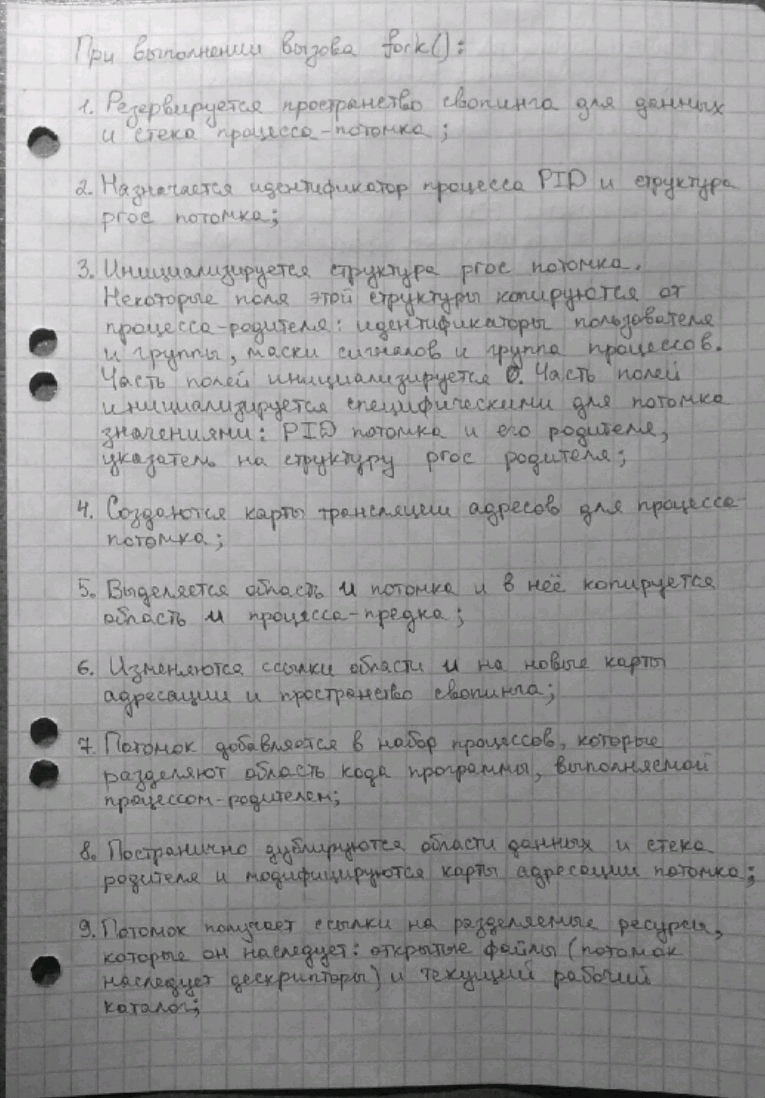
\includegraphics[width=0.7\linewidth]{img/fork1.jpg}
	\caption{Алгоритм работы системного вызова fork (Часть 1).}
\end{figure}

\begin{figure}[ht]
	\centering
	
\includegraphics[width=0.7\linewidth]{img/fork2.jpg}
	\caption{Алгоритм работы системного вызова fork (Часть 2).}
\end{figure}

\clearpage

\section{exec}

\begin{figure}[ht]
	\centering
	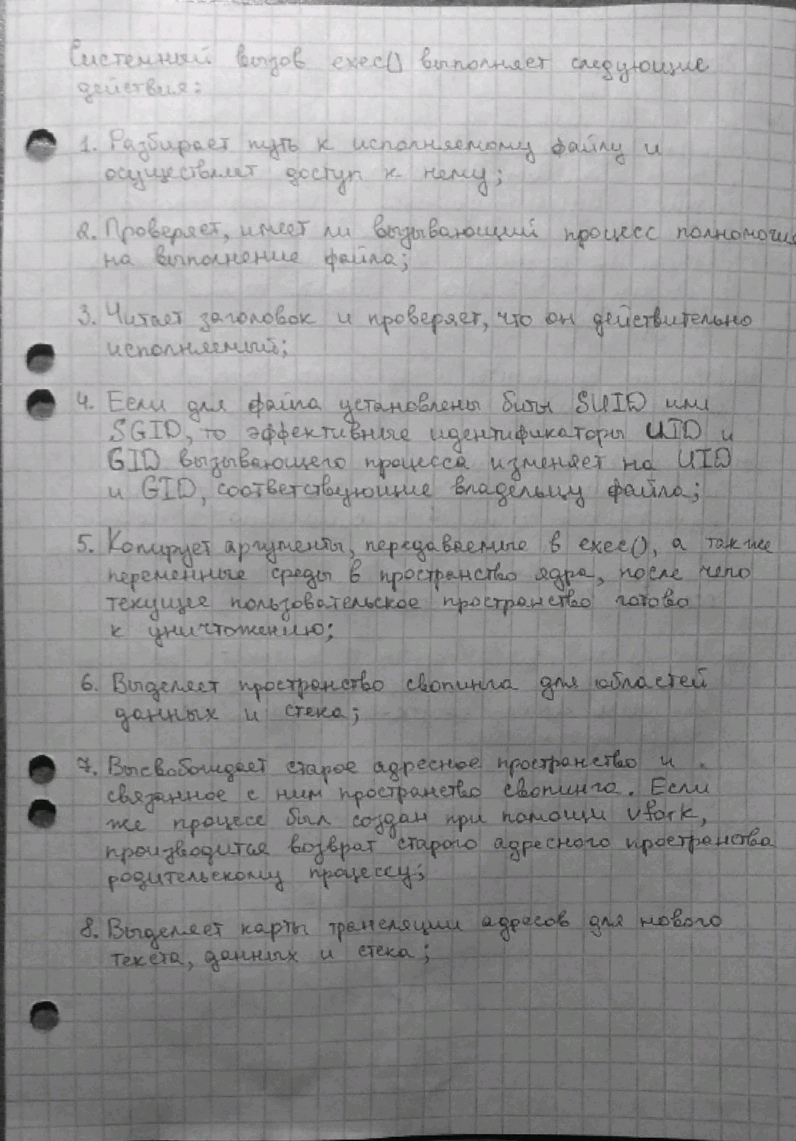
\includegraphics[width=0.7\linewidth]{img/exec1.jpg}
	\caption{Алгоритм работы системного вызова exec (Часть 1).}
\end{figure}

\begin{figure}[ht]
	\centering
	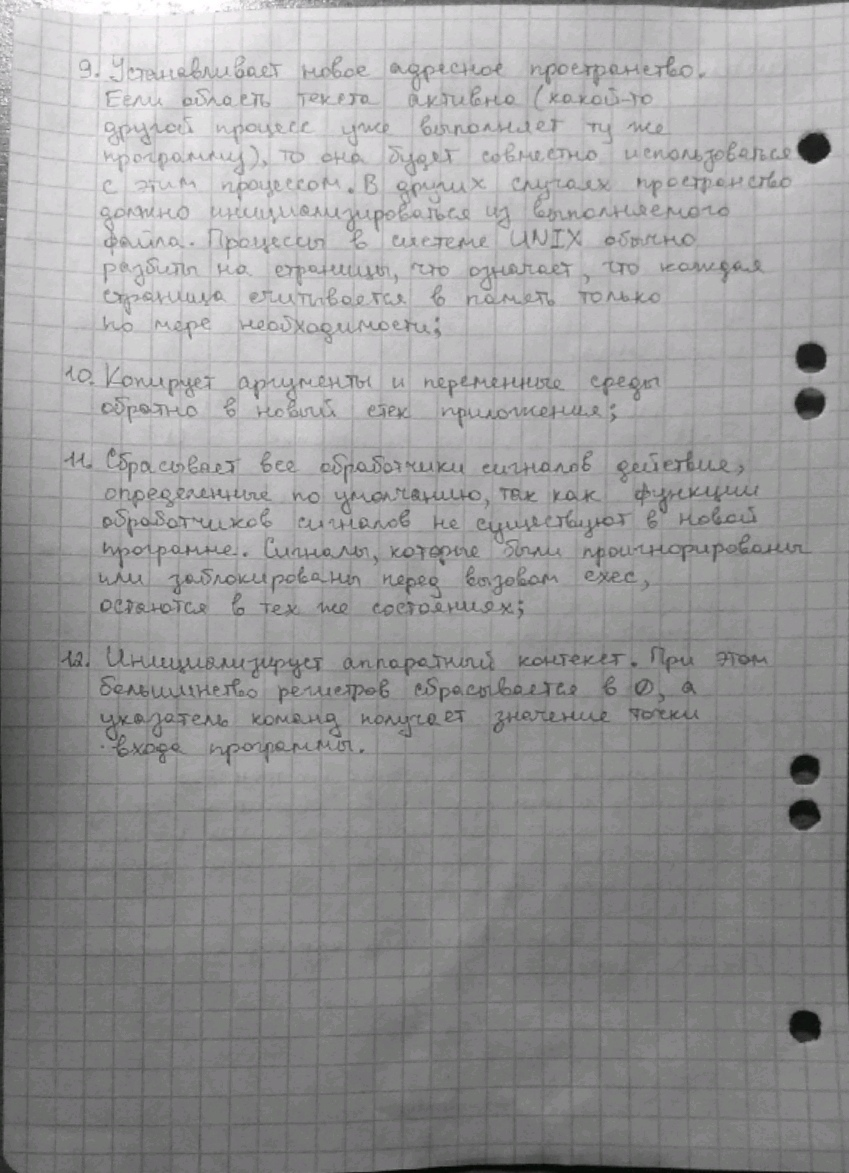
\includegraphics[width=0.7\linewidth]{img/exec2.jpg}
	\caption{Алгоритм работы системного вызова exec (Часть 2).}
\end{figure}

\clearpage

\chapter{Задания}

\section{Задание 1}

Написать программу, запускающую не менее двух новых процессов системным вызовом fork(). В предке вывести собственный идентификатор, идентификатор группы и идентификаторы потомков. В процессе-потомке вывести собственный идентификатор, идентификатор предка и идентификатор группы. Убедиться, что при завершении процесса-предка потомок, который продолжает выполняться, получает идентификатор предка (PPID), равный 1 или идентификатор процесса-посредника. В потомках вызывается sleep(). Чтобы предок гарантированно завершился раньше своих потомков. Продемонстрировать с помощью соответствующего вывода информацию об идентификаторах процессов и их группе. Продемонстрировать «усыновление». Для этого надо в потомках вывести идентификаторы: собственный, предка, группы до блокировки и после блокировки.

\begin{lstlisting}[language=C,caption=Исходный код для задания 1]
#include <stdio.h>
#include <stdlib.h>
#include <unistd.h>
#include <sys/types.h>

int main(void) {
	printf("Предок:  pid=%d gid=%d\n", getpid(), getpgrp());
	
	for (size_t i = 0; i < 5; i++) {
		pid_t child_pid = fork();
		if (child_pid == -1) {
			printf("Не удалось выполнить fork().\n");
			exit(EXIT_FAILURE);
		} else if (child_pid == 0) {
			printf("Потомок: pid=%d ppid=%d gid=%d\n", getpid(), getppid(), getpgrp());
			sleep(1);
			printf("pid=%d ppid=%d gid=%d\n", getpid(), getppid(), getpgrp());
			exit(EXIT_SUCCESS);
		}
	}
	
	return EXIT_SUCCESS;
}
\end{lstlisting}

\begin{figure}[ht]
	\centering
	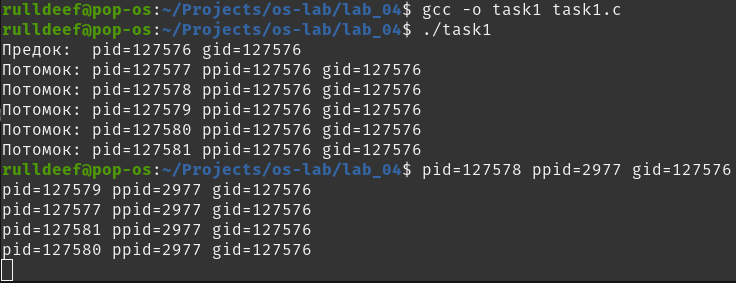
\includegraphics[width=\linewidth]{img/task1.png}
	\caption{Скриншот, демонстрирующий работу программы.}
\end{figure}

\clearpage

\section{Задание 2}

написать программу по схеме первого задания, но в процессе-предке выполнить системный вызов wait(). Убедиться, что в этом случае идентификатор процесса потомка на 1 больше идентификатора процесса-предка.

Предок ждет завершения своих потомком, используя системный вызов wait(). Вывод соответствующих сообщений на экран. В программе необходимо, чтобы предок выполнял анализ кодов завершения потомков.

\begin{lstlisting}[language=C,caption=Исходный код для задания 2.]
#include <stdio.h>
#include <stdlib.h>
#include <unistd.h>
#include <sys/types.h>
#include <sys/wait.h>

int main(void) {
	printf("Предок: pid=%d gid=%d\n", getpid(), getpgrp());
	
	for (size_t i = 0; i < 5; i++) {
		pid_t child_pid = fork();
		if (child_pid == -1) {
			printf("Не удалось выполнить fork().\n");
			exit(EXIT_FAILURE);
		} else if (child_pid == 0) {
			printf("Потомок #%ld: pid=%d ppid=%d gid=%d\n", i, getpid(), getppid(), getpgrp());
			exit(100 + i);
		}
	}
	
	for (size_t i = 0; i < 5; i++) {
		int status;
		pid_t child_pid = wait(&status);
		printf("Потомок с pid=%d ", child_pid);
		
		if (WIFEXITED(status))
			printf("завершился с кодом %d.\n", WEXITSTATUS(status));
		else if (WIFSIGNALED(status))
			printf("остановлен сигналом с кодом %d\n", WTERMSIG(status));
		else if (WIFSTOPPED(status))
			printf("остановлен с кодом %d\n", WSTOPSIG(status));
	}
	
	return EXIT_SUCCESS;
}
\end{lstlisting}

\begin{figure}[ht]
	\centering
	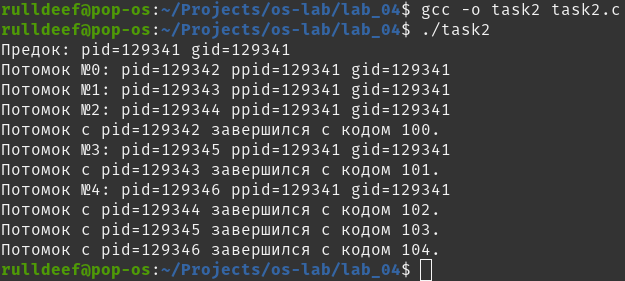
\includegraphics[width=\linewidth]{img/task2.png}
	\caption{Скриншот, демонстрирующий работу программы.}
\end{figure}

\clearpage

\section{Задание 3}

Написать программу, в которой процесс-потомок вызывает системный вызов exec(), а процесс-предок ждет завершения процесса-потомка. Следует создать не менее двух потомков.

Потомки переходят на выполнение других программ, которые передаются системному вызову exec() в качестве параметра. Потомки должны выполнять разные программы. Предок ждет завершения своих потомков с анализом кодов завершения. На экран выводятся соответствующие сообщения.

\begin{lstlisting}[language=C,caption=Исходный код для задания 3.]
#include <stdio.h>
#include <stdlib.h>
#include <unistd.h>
#include <sys/types.h>
#include <sys/wait.h>

void execute_program(const char* filepath, const char* filename, const char* arg);

int main(void) {
	execute_program("./lister", "lister", "list_in.txt");
	execute_program("./pysort.py", "pysort.py", "list_in.txt");
	return EXIT_SUCCESS;
}

void execute_program(const char* filepath, const char* filename, const char* arg) {
	pid_t child_pid = fork();
	
	if (child_pid == -1) {
		printf("Не удалось выполнить fork().\n");
		exit(EXIT_FAILURE);
	} else if (child_pid == 0)
		execl(filepath, filename, arg, NULL);
	
	int status;
	waitpid(child_pid, &status, 0);
	
	printf("Потомок с pid=%d ", child_pid);
	if (WIFEXITED(status))
		printf("завершился с кодом %d.\n", WEXITSTATUS(status));
	else if (WIFSIGNALED(status))
		printf("остановлен сигналом с кодом %d\n", WTERMSIG(status));
	else if (WIFSTOPPED(status))
		printf("остановлен с кодом %d\n", WSTOPSIG(status));
}
\end{lstlisting}

\begin{figure}[ht]
	\centering
	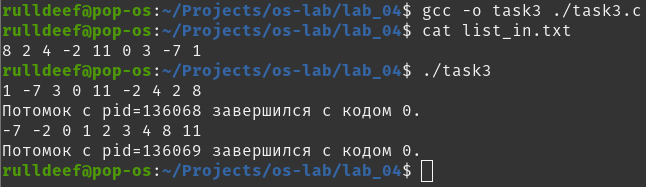
\includegraphics[width=\linewidth]{img/task3.png}
	\caption{Скриншот, демонстрирующий работу программы.}
\end{figure}

\clearpage

\section{Задание 4}

Написать программу, в которой предок и потомок обмениваются сообщением через программный канал. Причем оба потомка пишут свои сообщения в один программный канал, а предок их считывает из канала. Потомки должны посылать предку разные сообщения по содержанию и размеру. Предок считывает сообщения от потомков и выводит их на экран. Предок ждет завершения своих потомков и анализирует код их завершения. Вывод соответствующих сообщений на экран.

\begin{lstlisting}[language=C,caption=Исходный код для задания 4 (Часть 1).]
#include <stdio.h>
#include <stdlib.h>
#include <string.h>
#include <unistd.h>
#include <sys/types.h>
#include <sys/wait.h>

int main(void) {
	int pipefd[2];
	if (pipe(pipefd) == -1) {
		printf("Не удалось создать программный канал.\n");
		exit(EXIT_FAILURE);
	}
	
	const char* messages[] = {
		"Привет, я потомок.\n",
		"Жду указаний!\n",
		"А лаба будет?\n",
		"Будет\n"
	};
	size_t n = sizeof(messages) / sizeof(messages[0]);
	for (size_t i = 0; i < n; i++) {
		pid_t child_pid = fork();
		if (child_pid == -1) {
			printf("Не удалось выполнить fork().\n");
			exit(EXIT_FAILURE);
		} else if (child_pid == 0) {
			close(pipefd[0]); // закрытие канала для чтения
			write(pipefd[1], messages[i], strlen(messages[i]));
			exit(EXIT_SUCCESS);
		}
	}
\end{lstlisting}

\clearpage

\begin{lstlisting}[language=C,firstnumber=33,caption=Исходный код для задания 4 (Часть 2).]
	for (size_t i = 0; i < n; i++) {
		int status;
		pid_t child_pid = wait(&status);
		printf("Потомок с pid=%d ", child_pid);
		
		if (WIFEXITED(status))
			printf("завершился с кодом %d.\n", WEXITSTATUS(status));
		else if (WIFSIGNALED(status))
			printf("остановлен сигналом с кодом %d\n", WTERMSIG(status));
		else if (WIFSTOPPED(status))
			printf("остановлен с кодом %d\n", WSTOPSIG(status));
	}
	
	close(pipefd[1]); // закрытие канала на запись
	
	char buffer[256];
	read(pipefd[0], buffer, 256);
	printf("Предок получил сообщения от потомков:\n%s", buffer);
	
	return EXIT_SUCCESS;
}
\end{lstlisting}

\begin{figure}[ht]
	\centering
	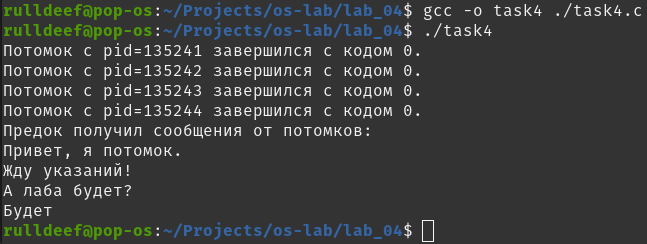
\includegraphics[width=\linewidth]{img/task4.png}
	\caption{Скриншот, демонстрирующий работу программы.}
\end{figure}

\clearpage

\section{Задание 5}

В программу с программным каналом включить собственный обработчик сигнала. Использовать сигнал для изменения хода выполнения программы.

Предок и потомки аналогично заданию 4 обмениваются сообщениями через неименованный программный канал. В программу включается собственный обработчик сигнала. С помощью сигнала меняется ход выполнения программы. При получении сигнала потомки записывают сообщения в канал, если сигнал не поступает, то не записывают. Предок ждет завершения своих потомков и анализирует коды их завершений. Вывод соответствующих сообщений на экран.

\begin{lstlisting}[language=C,caption=Исходный код для задания 5 (Часть 1).]
#include <stdio.h>
#include <stdlib.h>
#include <string.h>
#include <unistd.h>
#include <sys/types.h>
#include <sys/wait.h>
#include <sys/signal.h>

int write_enabled = 0;

void child_sig_handler(int sig) {
	write_enabled = 1;
}

int main(void) {
	int pipefd[2];
	if (pipe(pipefd) == -1) {
		printf("Не удалось создать программный канал.\n");
		exit(EXIT_FAILURE);
	}
	
	const char* messages[] = {
		"Привет, я потомок.\n",
		"Жду указаний!\n",
		"А лаба будет?\n",
		"Будет\n"
	};
	size_t n = sizeof(messages) / sizeof(messages[0]);
	for (size_t i = 0; i < n; i++) {
		pid_t child_pid = fork();
		if (child_pid == -1) {
			printf("Не удалось выполнить fork().\n");
			exit(EXIT_FAILURE);
\end{lstlisting}

\clearpage

\begin{lstlisting}[language=C,firstnumber=34,caption=Исходный код для задания 5 (Часть 2).]			
		} else if (child_pid == 0) {
			close(pipefd[0]); // закрытие канала для чтения
			// назначение обработчика сигнала для процесса-потомка
			signal(SIGINT, child_sig_handler);
			sleep(i);
			if (write_enabled)
				write(pipefd[1], messages[i], strlen(messages[i]));
			exit(EXIT_SUCCESS);
		}
	}
	
	close(pipefd[1]); // закрытие канала для записи
	// игнорирование сигнала SIGINT в родительском процессе
	signal(SIGINT, SIG_IGN);
	
	for (size_t i = 0; i < n; i++) {
		int status;
		pid_t child_pid = wait(&status);
		printf("Потомок с pid=%d ", child_pid);
		
		if (WIFEXITED(status))
			printf("завершился с кодом %d.\n", WEXITSTATUS(status));
		else if (WIFSIGNALED(status))
			printf("остановлен сигналом с кодом %d\n", WTERMSIG(status));
		else if (WIFSTOPPED(status))
			printf("остановлен с кодом %d\n", WSTOPSIG(status));
	}
	
	char buffer[256] = {'\0'};
	if (read(pipefd[0], buffer, 256))
		printf("Предок получил сообщения от потомков:\n%s", buffer);
	else
		printf("Предок не получил сообщений от потомков.\n");
	
	return EXIT_SUCCESS;
}
\end{lstlisting}

\begin{figure}[ht]
	\centering
	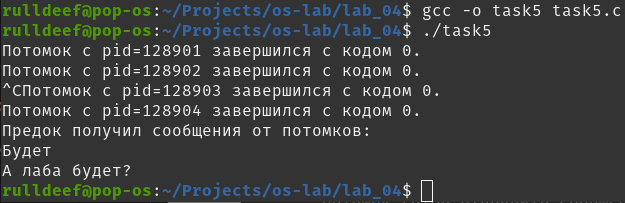
\includegraphics[width=\linewidth]{img/task5.png}
	\caption{Скриншот, демонстрирующий работу программы. В процессе работы программы был послан сигнал SIGINT.}
\end{figure}

\begin{figure}[ht]
	\centering
	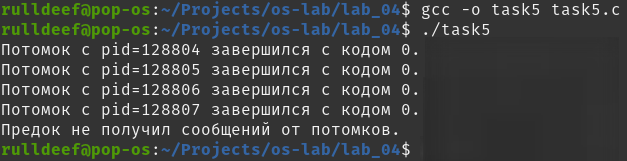
\includegraphics[width=\linewidth]{img/task5-2.png}
	\caption{Скриншот, демонстрирующий работу программы. В процессе работы программы сигналы не посылались.}
\end{figure}
